\documentclass[12pt]{article}

\usepackage{epsfig,array,amsmath,fancybox,epic}

\usepackage[latin1]{inputenc}

\voffset=-2cm
\hoffset=-1cm

\setlength{\textheight}{25cm}
\setlength{\textwidth}{16cm}
\setlength{\parindent}{0cm}

\renewcommand{\labelitemi}{\textbf{$\triangleright$}}
\renewcommand{\labelitemii}{\textbf{$\diamond$}}
\renewcommand{\labelitemiii}{\textbf{$\circ$}}
\renewcommand{\labelitemiv}{\textbf{$\cdot$}}

%-------------------------------------------------------------------------
\setlength{\fboxsep}{3mm}
%-------------------------------------------------------------------------

\begin{document}

\begin{LARGE}
\begin{bf}
\begin{center}
Biblioth\`eque de gestion\\
d'objets graphiques 2D
\end{center}
\end{bf}
\end{LARGE}

%-----------------------------------------------------------------------------

\section{Objectifs}

\vspace{0.3cm}
Ce projet a pour objet de faire d\'evelopper une application
compl\`ete, plus complexe que celles habituellement propos\'ees lors de
sujets de TP en temps limit\'e.

\vspace{0.2cm}
En laissant une grande part \`a l'initiative
des \'etudiants, ceux-ci pourront approfondir leur ma{\^\i}trise
du langage C, mettre en \'evidence leurs capacit\'es \`a trouver des
solutions originales mais \'egalement \^etre confront\'es aux probl\`emes de
complexit\'e de d\'eveloppement d'applications de moyenne envergure.

\vspace{0.2cm}
Ce projet pourra commencer par une familiarisation avec la
biblioth\`eque graphi\-que fournie \`a travers l'\'etude et la modification
d'un exemple fourni.

\vspace{0.2cm}
Ensuite les \'etudiants pourront choisir une
application de leur choix (casse-brique, circuit automobile,
tetris, tennis \ldots) et ils proposeront alors \`a l'enseignant une \'etude
de la solution envisag\'ee (sur papier, technique utilis\'ee, analyse
descendante \ldots). Une fois les \'etudiants et l'enseignant d'accord
sur la r\'ealisation \`a entreprendre, celle-ci pourra avoir lieu.

\vspace{0.2cm}
Un rapport pr\'esentant l'analyse du probl\`eme, les d\'etails de
r\'ealisation et les possibilit\'es d'\'evolution du logiciel fera
l'objet d'une \'evaluation.

%-----------------------------------------------------------------------------

\section{La biblioth\`eque graphique}

Dans le r\'epertoire \verb!LibObjects2D!
se trouvent des fichiers et r\'epertoires
utiles au d\'eveloppe\-ment de votre application.
Le fichier d'interface (\verb!LibObjects2D/include/CObject2D.h!)
donne acc\`es \`a une biblioth\`e\-que vous
permettant de manipuler des \verb!Object2D!s. Il s'agit d'un type
opaque d\'ecrivant un objet graphique situ\'e dans un plan $(x,y,\theta)$
structur\'e en couches (avant/arri\`ere-plan).

\begin{figure}[hbtp]
\begin{center}
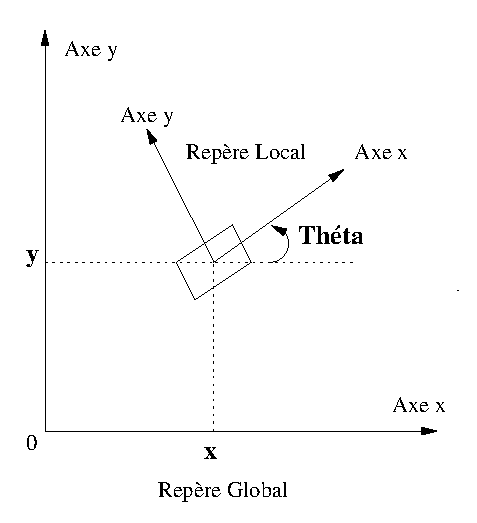
\includegraphics[width=5.8cm]{fig/reperes}
\end{center}
\caption{Description du rep\`ere global et du rep\`ere local associ\'e
\`a un objet graphique} 
\end{figure}

\newpage
Le lecteur trouvera dans la suite de cette section les fonctions qui sont
associ\'ees \`a ce type de donn\'ee.

\subsection{Fonctions de Cr\'eation/destruction/copie}

\begin{itemize}
\item \verb!Object2D *! \\
      \verb!Object2D_new(void);!
      \begin{itemize}
      \item Instancier un \verb!Object2D!.
      \item Sa repr\'esentation est un point blanc.
      \item Il se trouve sur la couche de visualisation $0$.
      \item Sa situation absolue sur le plan est $(x=0,y=0,\theta=0)$
      \end{itemize}

\item \verb!Object2D *! \\
      \verb!Object2D_newCopy(const Object2D * anObj2d);!
      \begin{itemize}
      \item Instancier un \verb!Object2D!.
      \item Sa repr\'esentation est celle de l'\verb!Object2D! pass\'e
            en param\`etre.
      \end{itemize}

\item \verb!void! \\
      \verb!Object2D_copy(Object2D * obj2d, const Object2D * anObj2d);!
      \begin{itemize}
      \item  Copier \verb!anObj2d! dans \verb!obj2d!
            (c'est-\`a-dire $\simeq$ \verb!*obj2d = *anObj2d!).
      \end{itemize}

\item \verb!void! \\
      \verb!Object2D_delete(Object2D * obj2d);!
      \begin{itemize}
      \item D\'etruire \verb!obj2d!.
      \end{itemize}

\end{itemize}

\subsection{Fonctions de gestion de la position et de l'orientation}

\begin{itemize}

\item \verb!void! \\
      \verb!Object2D_setLocation(Object2D * obj2d,! \\
      \verb!                     double x, double y,! \\
      \verb!                     double theta);!
      \begin{itemize}
      \item Situer \verb!obj2d! en absolu dans le plan.
      \end{itemize}

\item \verb!void! \\
      \verb!Object2D_getLocation(const Object2D * obj2d,! \\
      \verb!                     double * xOut, double * yOut,! \\
      \verb!                     double * thetaOut);!
      \begin{itemize}
      \item Obtenir la siuuation absolue d'\verb!obj2d! dans le plan.
      \end{itemize}

\item \verb!void! \\
      \verb!Object2D_setX(Object2D * obj2d,! \\
      \verb!              double x);!
      \begin{itemize}
      \item Fixer l'abscisse absolue d'\verb!obj2d! dans le plan.
      \end{itemize}

\item \verb!double! \\
      \verb!Object2D_getX(const Object2D * obj2d);!
      \begin{itemize}
      \item Obtenir l'abscisse absolue d'\verb!obj2d! dans le plan.
      \end{itemize}

\item \verb!void! \\
      \verb!Object2D_setY(Object2D * obj2d,! \\
      \verb!              double x);!
      \begin{itemize}
      \item Fixer l'ordonn\'ee absolue d'\verb!obj2d! dans le plan.
      \end{itemize}
\item \verb!double! \\
      \verb!Object2D_getY(const Object2D * obj2d);!
      \begin{itemize}
      \item Obtenir l'ordonn\'ee absolue d'\verb!obj2d! dans le plan.
      \end{itemize}
\item \verb!void! \\
      \verb!Object2D_setTheta(Object2D * obj2d,! \\
      \verb!                  double theta);!
      \begin{itemize}
      \item Fixer l'orientation absolue d'\verb!obj2d! dans le plan.
      \end{itemize}
\item \verb!double! \\
      \verb!Object2D_getTheta(const Object2D * obj2d);!
      \begin{itemize}
      \item Obtenir l'orientation absolue d'\verb!obj2d! dans le plan.
      \end{itemize}
\item \verb!void! \\
      \verb!Object2D_translate(Object2D * obj2d,! \\
      \verb!                   double dx, double dy);!
      \begin{itemize}
      \item Translation relative d'\verb!obj2d!.
      \item \verb!dx! et \verb!dy! sont exprim\'es dans le rep\`ere
            local d'\verb!obj2d!.
      \end{itemize}
\item \verb!void! \\
      \verb!Object2D_rotate(Object2D * obj2d,! \\
      \verb!                double dTheta);!
      \begin{itemize}
      \item Rotation relative d'\verb!obj2d!.
      \item \verb!dTheta! est exprim\'e dans le rep\`ere
            local d'\verb!obj2d!.
      \end{itemize}
\end{itemize}

\subsection{Fonctions de changements de rep\`eres (global/local)}

\begin{itemize}

\item \verb!void! \\
      \verb!Object2D_globalToLocalPosition(const Object2D * obj2d,! \\
      \verb!                               double * xInOut, double * yInOut);!
      \begin{itemize}
      \item Conversion d'une position globale dans un rep\`ere local.
      \item \verb!xInOut! et \verb!yInOut! sont exprim\'es dans le rep\`ere
            global en entr\'ee et dans le rep\`ere local d'\verb!obj2d! en
            sortie.
      \end{itemize}
\item \verb!void! \\
      \verb!Object2D_localToGlobalPosition(const Object2D * obj2d,! \\
      \verb!                               double * xInOut, double * yInOut);!
      \begin{itemize}
      \item Conversion d'une position locale dans le rep\`ere global.
      \item \verb!xInOut! et \verb!yInOut! sont exprim\'es dans le rep\`ere
            local d'\verb!obj2d! en entr\'ee et dans le rep\`ere global en
            sortie.
      \end{itemize}
\item \verb!double! \\
      \verb!Object2D_globalToLocalOrientation(const Object2D * obj2d,! \\
      \verb!                                  double orientation);!
      \begin{itemize}
      \item Conversion d'\verb!orientation! dans le rep\`ere local
            d'\verb!obj2d!.
      \item \verb!orientation! est exprim\'e dans le rep\`ere global.
      \end{itemize}
\item \verb!double! \\
      \verb!Object2D_localToGlobalOrientation(const Object2D * obj2d,! \\
      \verb!                                  double orientation);!
      \begin{itemize}
      \item Conversion d'\verb!orientation! dans le rep\`ere global.
      \item \verb!orientation! est exprim\'e dans le rep\`ere local
            d'\verb!obj2d!.
      \end{itemize}

\end{itemize}

\subsection{Fonctions de gestion de la couleur,
            de la couche de visualisation (layer) et de
            la forme des {\tt Object2D}}

\begin{itemize}

\item \verb!void! \\
      \verb!Object2D_setColor(Object2D * obj2d,!\\
      \verb!                  const char * colorName);!
      \begin{itemize}
      \item Modifier la couleur d'\verb!obj2d!.
      \item \verb!colorName! peut d\'esigner le nom d'une couleur
            (\verb!"blue"!, \verb!"grey"! \ldots) ou bien le motif
            \verb!"rgb:RR/GG/BB"! o\`u \verb!RR!, \verb!GG! et \verb!BB!
            sont les composantes de la couleur choisie exprim\'ees sur
            deux chiffres hexad\'ecimaux (\verb!00! \`a \verb!FF!).
      \end{itemize}
\item \verb!const char *! \\
      \verb!Object2D_getColor(Object2D * obj2d);!
      \begin{itemize}
      \item Obtenir la couleur d'\verb!obj2d!. Retourne \verb!NULL!
            si l'objet est invisible (cf {\tt noShape})
      \end{itemize}
\item \verb!void! \\
      \verb!Object2D_setLayer(Object2D * obj2d,!\\
      \verb!                  int layer);!
      \begin{itemize}
      \item Placer \verb!obj2d! sur une couche de visualisation.
      \item Les valeurs croissantes de \verb!layer! progressent vers
            l'avant-plan.
      \end{itemize}
\item \verb!int! \\
      \verb!Object2D_getLayer(const Object2D * obj2d);!
      \begin{itemize}
      \item Obtenir la couche de visualisation sur laquelle \'evolue
            \verb!obj2d!.
      \end{itemize}
\item \verb!void! \\
      \verb!Object2D_noShape(Object2D * obj2d);!
      \begin{itemize}
      \item \verb!obj2d! ne prend aucune forme... devient invisible !
      \end{itemize}
\item \verb!void! \\
      \verb!Object2D_point(Object2D * obj2d);!
      \begin{itemize}
      \item \verb!obj2d! prend la forme d'un point.
      \end{itemize}
\item \verb!void! \\
      \verb!Object2D_text(Object2D* obj2d, const char * text);!
      \begin{itemize}
      \item \verb!obj2d! prend la forme d'une cha{\^\i}ne de caract\`eres.
      \end{itemize}
\item \verb!void! \\
      \verb!Object2D_line(Object2D * obj2d,! \\
      \verb!              double length);!
      \begin{itemize}
      \item \verb!obj2d! prend la forme d'une ligne.
      \item La ligne va de $(0,0)$ \`a $(length,0)$ dans le rep\`ere local
            d'\verb!obj2d!.
      \end{itemize}
\item \verb!void! \\
      \verb!Object2D_square(Object2D * obj2d,! \\
      \verb!                double side,! \\
      \verb!                int filled);!
      \begin{itemize}
      \item \verb!obj2d! prend la forme d'un carr\'e.
      \item Le carr\'e est centr\'e en $(0,0)$ sur le rep\`ere local
            d'\verb!obj2d!, les cot\'es ont une longueur \verb!side!
            et sont orient\'es selon les axes du rep\`ere local
            d'\verb!obj2d!.
      \item Si \verb!filled! est non nul, le carr\'e est plein.
      \end{itemize}
\item \verb!void! \\
      \verb!Object2D_rectangle(Object2D * obj2d,! \\
      \verb!                   double length,! \\
      \verb!                   double width,! \\
      \verb!                   int filled);!
      \begin{itemize}
      \item M\^eme principe qu'avec \verb!Object2D_square()! mais pour
            un rectangle.
      \item \verb!length! et \verb!width! donnent respectivement la longueur
            selon l'axe $\vec{x}$ local et la largeur selon l'axe $\vec{y}$
            local.
      \end{itemize}
\item \verb!void! \\
      \verb!Object2D_polyline(Object2D * obj2d,! \\
      \verb!                  unsigned int nbPoints,! \\
      \verb!                  const double * xPoints,! \\
      \verb!                  const double * yPoints);!
      \begin{itemize}
      \item M\^eme principe qu'avec \verb!Object2D_line()! mais pour
            une ligne bris\'ee.
      \item Les coordonn\'ees $(x,y)$ sont exprim\'ees dans le rep\`ere
            local d'\verb!obj2d!.
      \end{itemize}
\item \verb!void! \\
      \verb!Object2D_polygon(Object2D * obj2d,! \\
      \verb!                 unsigned int nbPoints,! \\
      \verb!                 const double * xPoints,! \\
      \verb!                 const double * yPoints,! \\
      \verb!                 int filled);!
      \begin{itemize}
      \item M\^eme principe qu'avec \verb!Object2D_square()! mais pour
            un polygone.
      \item Les coordonn\'ees $(x,y)$ sont exprim\'ees dans le rep\`ere
            local d'\verb!obj2d!.
      \item Le dernier point et le premier point sont reli\'es.
      \end{itemize}
\item \verb!void! \\
      \verb!Object2D_circle(Object2D * obj2d,! \\
      \verb!                double radius,! \\
      \verb!                int filled);!
      \begin{itemize}
      \item M\^eme principe qu'avec \verb!Object2D_square()! mais pour
            un cercle.
      \end{itemize}
\item \verb|int /* 0: failure    !=0: success */| \\
      \verb!Object2D_image(Object2D * obj2d,! \\
      \verb!               const char * fileName,! \\
      \verb!               double pixelScale);!
      \begin{itemize}
      \item M\^eme principe qu'avec \verb!Object2D_square()! mais pour
            une image.
      \item Le fichier \verb!fileName! doit \^etre au format \verb!bmp!
            ou \verb!ras! et utiliser une pallette (pas d'image 24 bits).
      \item \verb!pixelScale! indique la taille d'un pixel de l'image
            dans le plan.
      \item Retourne un r\'esultat nul si le fichier n'est pas au format
            attendu.
      \end{itemize}
\item \verb!int /* 0: failure    !=0: success */! \\
      \verb!Object2D_getImagePixelAt(Object2D * obj2d,! \\
      \verb!                         double x,! \\
      \verb!                         double y,! \\
      \verb!                         int * redOut,! \\
      \verb!                         int * greenOut,! \\
      \verb!                         int * blueOut);!
      \begin{itemize}
      \item Donne la couleur du pixel qui se trouve en $(x,y)$ dans le plan
            (rep\`ere global).
      \item Retourne un r\'esultat nul si \verb!obj2d! n'a pas la forme d'une
            image ou si $(x,y)$ n'est pas \`a l'int\'erieur d'\verb!obj2d!.
      \end{itemize}
\end{itemize}

\subsection{Fonctions de d\'etection de repr\'esentations graphiques} 

\begin{itemize}
\item \verb|int /* 0: outside    !=0: inside */| \\
      \verb!Object2D_isInside(const Object2D * obj2d,! \\
      \verb!                  double x, double y);!
      \begin{itemize}
      \item Non nul si le point $(x,y)$ est situ\'e \`a l'int\'erieur de la
            repr\'esentation d'\verb!obj2d!.
      \item \verb!x! et \verb!y! sont exprim\'es dans le rep\`ere global.
      \end{itemize}
\item \verb|int /* 0: no intersection found   !=0: intersection found */| \\
      \verb!Object2D_intersectRay(const Object2D * obj2d,! \\
      \verb!                      double xRay, double yRay,!\\
      \verb!                      double thetaRay,!\\
      \verb!                      double * xOut,!\\
      \verb!                      double * yOut);!
      \begin{itemize}
      \item Non nul si la repr\'esentation d'\verb!obj2d! est intersect\'ee
            par la demi-droite issue de $(xRay,yRay)$ et orient\'ee selon
            $thetaRay$.
      \item \verb!xOut! et \verb!yOut! re\c coivent alors le point d'intersection.
      \item \verb!xRay!, \verb!yRay!, \verb!thetaRay!, \verb!xOut! et
            \verb!yOut! sont exprim\'es dans le rep\`ere global.
      \end{itemize}

\item \verb!Object2D * /* NULL: no intersection found, not NULL: intersection found */! \\
      \verb!Object2D_throwRay(const Object2D * obj2d,! \\
      \verb!                  double * xOut,!\\
      \verb!                  double * yOut,! \\
      \verb!                  Object2D *tabObject2D[], unsigned int nbObject2D);!
      \begin{itemize}
      \item Lance un rayon devant l'objet \verb!obj2d!
      (via les coordonnees et l'axe de \verb!obj2d!).
      \item Retourne l'objet le plus proche intersect\'e par ce rayon
      (object contenu dans le tableau \verb!tabObject2D!, tableau de
      \verb!nbObject2D! \'el\'ements).
      \item Retourne \verb!NULL! si pas d'objet intersect\'e.
      \item \verb!xOut! et \verb!yOut! re\c coivent alors le point
      d'intersection.
      \item \verb!xOut! et \verb!yOut! sont exprim\'es dans le rep\`ere global.
      \end{itemize}
\end{itemize}

\subsection{Fonctions de d\'etection d'objets dans un c\^one de vision}

Contrairement aux fonctions de d\'etection de repr\'esentations graphiques
qui travaillent sur les formes 2D des objets, les fonctions pr\'esent\'ees
dans cette sous-section travaillent sur les positions ({\tt x},{\tt y}) des
objets.

Ces fonctions utilisent la notion de c\^one de vision.
Ainsi, pour un {\tt Object2D} {\tt obj2d}, un c\^one de vision est
d\'etermin\'e par 3 r\'eels {\tt vision}, {\tt range} et {\tt turn}.

\begin{figure}[hbtp]
\begin{center}
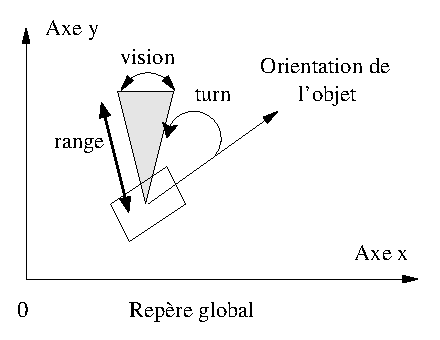
\includegraphics[width=7.5cm]{fig/cone}
\end{center}
\caption{C\^one de d\'etection d'un object en fonction de son l'orientation
et des param\`etres {\tt vision}, {\tt range} et {\tt turn}.
Si {\tt range} est \'egal \`a {\tt 0.0} $\Longrightarrow$ range~: $\infty$.}
\end{figure}

\begin{itemize}

\item \verb!Object2D * /* NULL: no Object2D found, not NULL: an Object2D */!\\
      \verb!Object2D_viewFirstObject2D(const Object2D * obj2d,!\\
      \verb!                           double vision, double range, double turn);!
      \begin{itemize}
      \item Retourne l'{\tt Object2D} le plus proche se trouvant dans le
            c\^one de vision de l'object {\tt obj2d}, c\^one de vision
            d\'etermin\'e par {\tt vision}, {\tt range} et {\tt turn}.
      \item Si {\tt range} est \'egal \`a {\tt 0.0}
            $\Longrightarrow$ range~: $\infty$
      \end{itemize}

\item \verb!int!\\
      \verb!Object2D_viewObject2D(const Object2D * obj2d,!\\
      \verb!                      Object2D*** tabObject2D,!\\
      \verb!                      double vision, double range, double turn);!
      \begin{itemize}
      \item Retourne le nombre d'{\tt Object2D} se trouvant dans le
            c\^one de vision de l'object {\tt obj2d},
            c\^one de vision d\'etermin\'e par {\tt vision}, {\tt range}
            et {\tt turn}.
            A la sortie de la fonction, les objets se trouvant dans
            ce c\^one de vision sont disponibles dans un tableau allou\'e
            dynamiquement (avec {\tt malloc})...
            il faudra penser \`a faire un {\tt free}~!
      \item Si {\tt range} est \'egal \`a {\tt 0.0}
            $\Longrightarrow$ range~: $\infty$
      \item Exemple d'utilisation~:
            
\begin{small}
\begin{verbatim}
void testViewObject2D(Object2D* obj2d)
{
 double range = 10;

 Object2D** v;
 int i, nbObj2D;

 nbObj2D = Object2D_viewObject2D(obj2d,&v,2*M_PI,range,0.0);

 for(i=0;i<nbObj2D;i++)
 {
  v[i]->setColor("yellow");
 }

 free(v);  /* Important (autrement, il y a une fuite memoire !) */
}
\end{verbatim}
\end{small}

Dans cet exemple, tous les objets se trouvant \`a une distance
inf\'erieure \`a {\tt 10} de {\tt obj2d} sont d\'etect\'es...
Et deviennent jaunes.

      \end{itemize}
\end{itemize}

\subsection{Fonction d'interaction ``clavier''/``souris''}

\begin{itemize}

\item \verb!void! \\
      \verb!Object2D_onKeyPress(Object2D * obj2d, const char * key);!
      \begin{itemize}
      \item Ex\'ecute le comportement par defaut d'un Object2D lorsque
            celui-ci est s\'electionn\'e et qu'une touche est appuy\'ee.\\
            Par exemple, affichage de \verb!Object 0x100fe080 key <f>!.
      \end{itemize}

\vspace{0.2cm}
\item \verb!void! \\
      \verb!Object2D_onMouseDrag(Object2D * obj2d, double dx, double dy);!
      \begin{itemize}
      \item Ex\'ecute le comportement par defaut d'un Object2D lorsque
            celui-ci est d\'eplac\'e \`a la souris de ({\tt dx},{\tt dy}).
\vspace{0.1cm}
      \item Cela revient \`a~:
\begin{small}
\begin{verbatim}
void
Object2D_onMouseDrag(Object2D * obj2d, double dx, double dy)
{
 double x,y,theta;

 Object2D_getLocation(&x,&y,&theta);
 x+=dx;
 y+=dy;
 Object2D_setLocation(x,y,theta);
}
\end{verbatim}
\end{small}
      \end{itemize}

\end{itemize}

\vspace{0.15cm}
\subsection{Fonction de gestion de l'attachement d'objets ensemble}

\vspace{0.3cm}
\begin{itemize}
\item \verb!void!\\
      \verb!Object2D_attachTo(Object2D * obj2d, const Object2D * anObj2d);!
      \begin{itemize}
      \item L'Object2D \verb!obj2d! est attach\'e \`a l'Object2D
            \verb!anObj2d!.\\
            $\Longrightarrow$ Lors d'un d\'eplacement de \verb!anObj2d!, 
            \verb!obj2d! subit le m\^eme d\'eplacement.
            $\Longrightarrow$ L'inverse n'est pas vrai...
      \end{itemize}
\vspace{0.1cm}
\item \verb!int /* 0: no    1: yes */! \\
      \verb!Object2D_isAttachedTo(const Object2D * obj2d,!\\
      \verb!                      const Object2D * anObj2d);!
      \begin{itemize}
      \item Permet de savoir si l'Object2D \verb!obj2d! est attach\'e
            \`a l'Object2D \verb!anObj2d!.
      \item ... permet de savoir si on a fait un
        \verb!Object2D_attachTo(obj2d,anObj2d);!
      \end{itemize}
\vspace{0.1cm}
\item \verb!void! \\
      \verb!Object2D_detachFrom(Object2D * obj2d, const Object2D * anObj2d);!
      \begin{itemize}
      \item Supprime l'attachement de l'Object2D \verb!obj2d! \`a
            l'Object2D \verb!anObj2d!.
      \item ... op\'eration inverse de \verb!Object2D_attachTo(obj2d,anObj2d);!
      \end{itemize}
\vspace{0.1cm}
\item \verb!void! \\
      \verb!Object2D_detachFromAll(Object2D * obj2d);!
      \begin{itemize}
      \item Supprime tous les attachements r\'ealis\'e par l'Object2D
       \verb!obj2d!.
      \end{itemize}
\end{itemize}


%---------------------------------------------------------------

\newpage
\section{Initialisation, activation et param\'etrage de\\
         l'application graphique}

Le fichier d'interface \verb!LibObjects2D/include/CObject2D.h!
donne \'egalement acc\`es \`a des fonctions
permettant d'initialiser et d'activer l'application graphique~:

\begin{itemize}
\item \verb!void! \\
      \verb!graphic_init(const char * windowName,! \\
      \verb!             const char * fontName);!
      \begin{itemize}
      \item Cr\'eer la fen\^etre graphique en lui affectant le titre
            \verb!windowName!.
      \item Les \verb!Object2D!s ayant une repr\'esentation sous forme
            de texte utiliseront la police \verb!fontName!.
      \item Cette fonction doit \^etre appel\'ee avant toutes les autres
            fonctions de la bi\-blio\-th\`eque.
      \end{itemize}
\item \verb!void! \\
      \verb!graphic_setWidth(int width);!
      \begin{itemize}
      \item Fixer la largeur en pixels de la fen\^etre graphique.
      \end{itemize}
\item \verb!void! \\
      \verb!graphic_setHeight(int height);!
      \begin{itemize}
      \item Fixer la hauteur en pixels de la fen\^etre graphique.
      \end{itemize}
\item \verb!void! \\
      \verb!graphic_setBackground(const char * colorName);!
      \begin{itemize}
      \item Changer la couleur du fond de la fen\^etre graphique.
      \end{itemize}
\item \verb!void! \\
      \verb!graphic_setViewPoint(double x,! \\
      \verb!                     double y,! \\
      \verb!                     double scale);!
      \begin{itemize}
      \item Modifier le point de vue de la fen\^etre
      \item Le point $(x,y)$ repr\'esente le point du plan qui sera situ\'e
            au centre de la fen\^etre.
      \item \verb!scale! repr\'esente le facteur qui permet de passer des
            grandeurs sans dimension du plan aux \textit{pixels} de l'\'ecran.
      \end{itemize}
\item \verb!void! \\
      \verb!graphic_getViewPoint(double * xOut,! \\
      \verb!                     double * yOut,! \\
      \verb!                     double * scaleOut);!
      \begin{itemize}
      \item Obtenir le point de vue courant de la fen\^etre.
      \item Voir \verb!graphic_setViewPoint()! .
      \end{itemize}
\item \verb!void! \\
      \verb!graphic_autoscale(void);!
      \begin{itemize}
      \item Recadrer la fen\^etre pour qu'elle montre
            l'ensemble des \verb!Object2D!s.
      \end{itemize}
\end{itemize}
\newpage
\begin{itemize}
\item \verb!void! \\
      \verb!graphic_run(void * userData);!
      \begin{itemize}
      \item Lancer la partie active (\'ev\'enementielle) du programme.
      \item \verb!userData! d\'esigne g\'en\'eralement une structure
            cr\'e\'ee par vos soins, permettant d'acc\'eder \`a l'ensemble
            des donn\'ees de l'application.
      \end{itemize}
\item \verb!void! \\
      \verb!graphic_mainLoop(void * userData);!
      \begin{itemize}
      \item Cette fonction est appel\'ee perp\'etuellement \`a partir
            de \verb!graphic_run()!~; c'est la cin\'ematique de l'application.
      \item \textbf{Vous devez d\'efinir cette fonction !}
      \item Le param\`etre \verb!userData! est celui qui a \'et\'e
            transmis \`a \verb!graphic_run()!.
      \end{itemize}
\item \verb!void! \\
      \verb!graphic_keyPressCallback(Object2D * obj2d,! \\
      \verb!                         const char * key,! \\
      \verb!                         void * userData);!
      \begin{itemize}
      \item Cette fonction est appel\'ee lorsqu'une touche du clavier est
            enfonc\'ee.
      \item \textbf{Vous devez d\'efinir cette fonction !}
      \item Si \verb!obj2d! est non nul, il s'agit d'un objet graphique
            qui \'etait s\'electionn\'e lors de l'appui sur la touche.
      \item Si \verb!obj2d! est nul, aucun objet graphique n'\'etait
            s\'electionn\'e au moment de l'appui sur la touche.
      \item La touche enfonc\'ee est d\'ecrite de mani\`ere lisible par
            \verb!key!.
      \item Le param\`etre \verb!userData! est celui qui a \'et\'e
            transmis \`a \verb!graphic_run()!.
      \end{itemize}
\item \verb!void! \\
      \verb!graphic_mouseDragCallback(Object2D * obj2d,! \\
      \verb!                          double dx,! \\
      \verb!                          double dy,! \\
      \verb!                          void * userData);!
      \begin{itemize}
      \item Cette fonction est appel\'ee lorsqu'un mouvement de souris
            est appliqu\'e \`a un \verb!Object2D!.
      \item \textbf{Vous devez d\'efinir cette fonction !}
      \item \verb!obj2d! d\'esigne l'objet s\'electionn\'e lors du
            mouvement de souris.
      \item Le mouvement est d\'ecrit par le vecteur $(dx,dy)$ dans le
            rep\`ere global.
      \item Le param\`etre \verb!userData! est celui qui a \'et\'e
            transmis \`a \verb!graphic_run()!.
      \end{itemize}
\end{itemize}

Tous les mouvements et les dimensions des \verb!Object2D! sont exprim\'es
dans une grandeur sans dimention~; ce ne sont pas des pixels.
L'axe $\vec{x}$ cro{\^\i}t de gauche \`a droite et l'axe $\vec{y}$ de bas
en haut. Le point de vue de la fen\^etre peut \^etre modifi\'e selon des
translations (\verb!Ctrl!+Click Gauche) et selon un facteur de grossissement
(\verb!Ctrl!+Click Droit).

\section{A savoir: quelques fonctions utilitaires}

La biblioth\`eque de gestion d'{\tt Object2D} fournit \'egalement quelques
fonctions utilitaires concernant le passage de coordonn\'ees
cart\'esiennes en coordonn\'ees polaires (et inversement), ... et
d'autres fonctions d\'ecrites ci-apr\`es.
\begin{center}
voir le fichier {\tt LibObjects2D/include/UtilObject2D.h}
\end{center}

\begin{figure}[h]
\begin{center}
\includegraphics[width=3.5cm]{fig/cartPolaire}
\end{center}
\vspace{-0.5cm}
\caption{Rappel~: coordonn\'ees cart\'esiennes ({\tt x},{\tt y})
-- coordonn\'ees polaires ({\tt d},{\tt th\'eta})}
\end{figure}

\begin{itemize}
\item \verb!void cartesianToPolar(double x,! \\
      \verb!                      double y,! \\
      \verb!          double * distanceOut,! \\
      \verb!          double * angleOut);!
      \begin{itemize}
      \item Cette fonction permet de passer des coordonn\'ees
            cart\'esiennes ({\tt x},{\tt y}) aux coordonn\'ees
            polaires ({\tt distanceOut},{\tt angleOut}).
      \end{itemize}

\item \verb!void polarToCartesian(double distance,!\\
      \verb!                      double angle,!\\
      \verb!                      double * xOut,!\\
      \verb!                      double * yOut);!
      \begin{itemize}
      \item Cette fonction permet de passer des coordonn\'ees
            polaires ({\tt distance},{\tt angle}) aux coordonn\'ees 
            cart\'esiennes ({\tt xOut},{\tt yOut})
      \end{itemize}

\item \verb!double cartToDist(double x,double y);!
      \begin{itemize}
      \item Cette fonction permet de passer des coordonn\'ees
            cart\'esiennes ({\tt x},{\tt y}) aux coordonn\'ees
            polaires.
      \item Dans cette fonction, il n'y a que le calcul de la distance.
      \item Cette fonction retourne la distance ainsi calcul\'ee.
      \end{itemize}

\item \verb!double cartToAngle(double x,double y);!
      \begin{itemize}
      \item Cette fonction permet de passer des coordonn\'ees
            cart\'esiennes ({\tt x},{\tt y}) aux coordonn\'ees
            polaires.
      \item Dans cette fonction, il n'y a que le calcul de l'angle.
      \item Cette fonction retourne l'angle ainsi calcul\'e.
      \end{itemize}

\item \verb!double betweenPi(double a);!
      \begin{itemize}
      \item Cette retourne, \`a partir d'un angle {\tt a},
            une valeur comprise entre $-\pi$ et $\pi$.
      \item Exemple~: si {\tt a} est \'egal \`a $\frac{5}{4}\pi$,
            la valeur retourn\'ee sera ~: $-\frac{3}{4}\pi$.
      \end{itemize}


\end{itemize}

%-----------------------------------------------------------------------------

\newpage

\section{L'exemple fourni}

Le fichier \verb!graphTestC.c! est un programme qui utilise de nombreuses
fonctionnalit\'es de la biblioth\`eque graphique. On y trouve trait\'e
un certain nombre de points qui pourront vous guider dans votre
r\'ealisation~:
\begin{itemize}
\item Squelette g\'en\'eral de l'application.
\item Fonctions utilitaires (temps, al\'eatoire \ldots).
\item Utilisation des formes, des couleurs \ldots
\item Changement de rep\`ere, suivi de cible.
\item Cadencement de l'application (mesure du temps).
\item Lancers de rayons.
\item Interactions clavier/souris.
\item Lecture des couleurs d'une image.
\item \ldots
\end{itemize}
Le \verb!Makefile! qui l'accompagne vous sera \'egalement utile pour vos
d\'eveloppements.
Vous pourrez constater sur certaines machines peu puissantes que
l'utilisation d'images est beaucoup plus p\'enalisante que l'utilisation
d'autres repr\'esentations. \'Evitez donc autant que possible d'y avoir
recours et limitez vous \`a des images de petite taille (peu de pixels).

%-----------------------------------------------------------------------------

\section{Travail demand\'e}

Apr\`es avoir pris en main et manipul\'e l'exemple fourni, choisissez le
programme graphique que vous souhaitez r\'ealiser. Proc\'edez \`a une analyse
descendante des fonctionnalit\'es en identifiant pour chaque traitement 
les entr\'es/sorties et les effets de bord. Apr\`es concertation avec
l'enseignant, la r\'ealisation pourra d\'ebuter. Elle donnera lieu \`a
plusieurs versions successives dans des r\'epertoires distincts (\verb!V1!,
\verb!V2! \ldots). Vous devrez rendre un rapport relatant l'analyse et les
d\'etails de r\'ealisation du projet.

\ifnum 1 = 1
\newpage
\section{Et pour ceux qui connaissent le C++}

\subsection{Contenu du fichier {\tt LibObjects2D/include/Object2D.h}}

\begin{small}
\begin{verbatim}
#ifndef   _OBJECT2D_H_
#define   _OBJECT2D_H_
\end{verbatim}
\begin{verbatim}
#include <vector>
#include <set>
#include <string>
#include <iostream>
\end{verbatim}
\begin{verbatim}
#include "guiTrans.h"
\end{verbatim}
\begin{verbatim}
#include "UtilObject2D.h"
\end{verbatim}
\begin{verbatim}
using namespace std;

class Object2D
{
 friend ostream& operator<<(ostream& os, const Object2D& object2D);

 public :

/*-------- Constructor/Destructor -----------------------------------------*/

         Object2D(void);
         Object2D(const Object2D& object2D);
virtual ~Object2D(void);

         Object2D& operator=(const Object2D& object2D);

 // Test d'egalite uniquement sur la couleur et le type de forme:
 // noShape, point, text, 
 friend   bool operator==(const Object2D& obj1, const Object2D& obj2);
 friend   bool operator!=(const Object2D& obj1, const Object2D& obj2);

/*-------- Location -------------------------------------------------------*/

      void   setLocation(double x, double y, double theta);
      void   getLocation(double& xOut, double& yOut, double& thetaOut) const;

      void   setX(double x);
      double getX(void) const;
      void   setY(double y);
      double getY(void) const;
      void   setTheta(double theta);
      double getTheta(void) const;

/*-------- Motion ---------------------------------------------------------*/

      void   translate(double dx, double dy);
      void   rotate(double dTheta);
/*-------- Interaction ----------------------------------------------------*/

virtual void onKeyPress(const char * key);
virtual void onMouseDrag(double dx, double dy);
\end{verbatim}
\begin{verbatim}
/*-------- Attachment -----------------------------------------------------*/

        void  attachTo(Object2D& object2D);
        bool  isAttachedTo(const Object2D& object2D) const;
        void  detachFrom(Object2D& object2D);
        void  detachFromAll(void);
\end{verbatim}
\begin{verbatim}
/*-------- Detection -------------------------------------------------------*/

      bool   isInside(double x, double y) const;
      bool   intersectRay(double xRay, double yRay, double thetaRay,
                          double& xOut, double& yOut) const;
      Object2D * throwRay(double& xOut, double& yOut,
                          Object2D *tabObject2D[],
                          unsigned int nbObject2D) const;

      Object2D * viewFirstObject2D(double vision,
                                   double range,
                                   double turn=0.0) const;
      int        viewObject2D(Object2D*** tabObject2D,         // Version C
                              double vision,
                              double range,
                              double turn=0.0) const;
      int        viewObject2D(vector<Object2D*>& vectObject2D, // Version C++
                              double vision,
                              double range,
                              double turn=0.0) const;
\end{verbatim}
\begin{verbatim}
/*-------- Transformation --------------------------------------------------*/

      void   globalToLocalPosition(double& xInOut, double& yInOut) const;
      void   localToGlobalPosition(double& xInOut, double& yInOut) const;

      double globalToLocalOrientation(double orientation) const;
      double localToGlobalOrientation(double orientation) const;
\end{verbatim}
\begin{verbatim}
/*-------- Representation --------------------------------------------------*/

      void   setColor(const char * colorName);
      const  char * getColor(void) const;// Retourne NULL si invisible(noShape)

      void   setLayer(int layer);
      int    getLayer(void) const;

      void   noShape(void);
      void   point(void);
      void   text(const char * text);
      void   line(double length);
\end{verbatim}
\newpage
\begin{verbatim}
      void   square(double side, int filled);
      void   rectangle(double length, double width, int filled);
      void   polyline(unsigned int nbPoints, const double * xPoints,
                                             const double * yPoints);
      void   polygon(unsigned int nbPoints,  const double * xPoints,
                                             const double * yPoints,
                                             int filled);
      void   circle(double radius, int filled);

      int    image(const char * fileName,        // 0: failure, !=0: success
                   double pixelScale);
      int    getImagePixelAt(double x, double y, // 0: failure, !=0: success
                             int& redOut,
                             int& greenOut,
                             int& blueOut);
      int    getImagePixelNumberAt(double x,     //  >=0: pixel number 
                                   double y);    //  <0: failure 
      int    setImagePixelNumberAt(int pixel,    // 0: failure, !=0: success
                                   double x,
                                   double y);
      int    getImageNbColors(void);             // number of colors
      int    getImageRGB(int pixel,              // 0: failure, !=0: success
                         int& redOut,
                         int& greenOut,
                         int& blueOut);

/*-------- Data types ------------------------------------------------------*/

 private : // ...

 protected:

  virtual void display(ostream& os) const;
  virtual bool isEqualTo(const Object2D& object2D) const;

           // ...
};

/*-------- Graphical application template ----------------------------------*/

extern void graphic_init(const char * windowName, const char * fontName);

extern void graphic_setWidth(int width);

extern void graphic_setHeight(int height);

extern void graphic_setBackground(const char * colorName);

extern void graphic_setViewPoint(double x, double y, double scale);

extern void graphic_getViewPoint(double * xOut, double * yOut,
                                 double *scaleOut);

extern void graphic_autoscale(void);

extern void graphic_run(void * userData);

extern void graphic_mainLoop(void * userData);

extern void graphic_keyPressCallback(Object2D * obj2d,
                                     const char * key,
                                     void * userData);

extern void graphic_mouseDragCallback(Object2D * obj2d,
                                      double dx, double dy,
                                      void * userData);

/*-------- Graphical application template --------*/
/*
   int
   main(void)
   {
   graphic_init("My Window","-*-helvetica-*-r-normal--14-*");
   graphic_setWidth(640);
   graphic_setHeight(480);
   ... application specific initializations ...
   graphic_run(myDataPointer);
   return(0);
   }

   void
   graphic_mainLoop(void * userData)
   {
   ...
   }

   void
   graphic_keyPressCallback(Object2D * obj2d,
                            const char * key,
                            void * userData)
   {
   ...
   }

   void
   graphic_mouseDragCallback(Object2D * obj2d,
                             double dx,
                             double dy,
                             void * userData)
   {
   ...
   }
*/
#endif // _OBJECT2D_H_
\end{verbatim}
\end{small}

\subsection{Contenu du fichier {\tt LibObjects2D/include/UtilObject2D.h}}

\begin{small}
\begin{verbatim}
#ifndef _UTILOBJECT2D_H_
#define _UTILOBJECT2D_H_

#include <math.h>

void cartesianToPolar(double x,
                      double y,
                      double * distanceOut,
                      double * angleOut);

void polarToCartesian(double distance,
                      double angle,
                      double * xOut,
                      double * yOut);

double cartToDist(double x,double y);

double cartToAngle(double x,double y);

double betweenPi(double a);

#endif // _UTILOBJECT2D_H_
\end{verbatim}
\end{small}

\fi  % ifnum pour \section{Et pour ceux qui connaissent le C++}

%\newpage

\section{Installation}

\vspace{-0.5cm}
\begin{figure}[hbtp]
\begin{center}
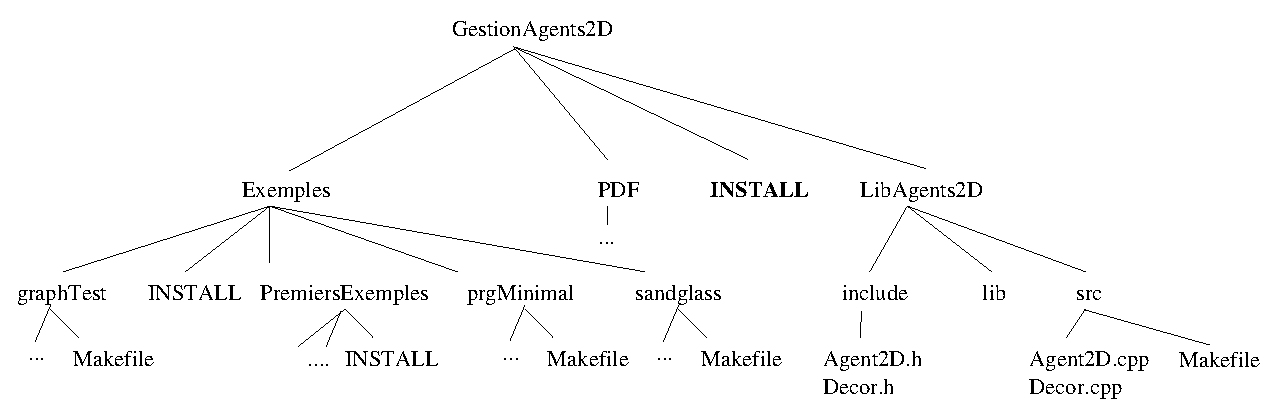
\includegraphics[width=15.5cm]{fig/arbo}
\end{center}
\caption{Description de l'arborescence de la biblioth\`eque}
\end{figure}

Aller dans le r\'epertoire {\tt LibObjects2D/lib}
et faire {\tt \$ make}

Une biblioth\`eque {\tt libObjects2D.a} est alors plac\'ee dans le r\'epertoire
{\tt LibObjects2D/lib}

Des exemples de programmes sont disponibles dans le r\'epertoire
{\tt Exemples}.

\vspace{0.5cm}
{\bf ... mais on peut faire plus simple !}

\vspace{0.3cm}

En \'etant dans le r\'epertoire {\tt GestionObjects2D}, faire tout
simplement {\tt \$ ./INSTALL}

Il faut ensuite aller dans les r\'epertoires avec les divers exemples
et faire {\tt \$ make}

\end{document}

